\chapter{Introduction}

\section{What is Cancer?}
Cancer is a collection of disease that is usually caused by uncontrolled division of cells and that has potential to spread to other parts of the body \cite{cancergov}. Cancer could be caused by various factors like tobacco usage, excess sun exposure, viral infection to name a few \cite{Trichopoulos}. Although, the underlying mechanism from these causes usually involves genetic mutations or epigenetic changes that alter the DNA. These alterations usually trigger a cascade of events that eventually leads to uncontrolled growth of cells \cite{Moolgavkar,Gronbaek}.

Cancer is among the highest causes of death among human beings. In the year 2021, over 600,000 deaths are expected to be caused by cancer in the US alone \cite{cancer_stats}. Cancer systems has been of research interest for several decades due to the massive impact it has on human lives. Through such research, we have been able to understand the causes and mechanism of how cancer arises and then develop new therapies and drugs that target them. Although, the mortality among some types of cancer have been reduced significantly, we were not so lucky among other types of cancers and, the overall mortality still remains pretty high.

\section{Conventional therapy against cancer}
The most popular strategies to control cancer are radiotherapy, chemotherapy, immunotherapy, and surgery. Depeneding on the type and stage of cancer, some of these strategies may not be effective.

Among chemotherapy, the standard clinical protocol, Standard of Care (SOC) followed for most cancer is to administer cytotoxic drugs at the maximum tolerated dosage (MTD) \cite{Frei}. The aim of this method is to kill the maximum number of tumour cells as fast as possible. This minimises the tumour burden quickly and should give better standard of living if it's the case.

However, evolutionarily thinking, a tumour would consist of cells with heterogenous sensitivity towards a cytotoxic drug. Under normal conditions, that is, in the absence of therapy, these cells would compete with each other and keep the number of resistant phenotype in check. On adminitering the drug at MTD, the most sensitive cells are killed off first and this leads to a ``competitive release" of the resistant phenotype \cite{Scott}. The resistant phenotype now grows without inhibition and takes over the population. These resistant phenotypes don't respond to further dose administered and the therapy fails. This is illustrated in \autoref{comperelease}.

Competitive release could happen for other methods of therapy as well, if there are resisitant phenotypes for that particular therapy method present in the population.

\begin{figure}[h]
  \centering
  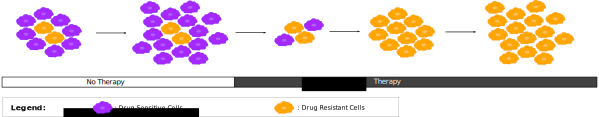
\includegraphics[width=\textwidth]{compe_release}
  \caption{Illustration of competitive release under SOC}
  \label{comperelease}
\end{figure}

\section{Adaptive therapy}
When competitive release happens, one could try to combat the cells with another drug or therapy method. However, these cells could potentially be resistant to the new drug as well and developing new drugs is research intensive. The best method would be to avoid such a competitive release in the first place.

Adaptive therapy (AT) is one such novel technique under development to avoid competitive release. In AT, the cytotoxic drug is administered at lower and fluctuating doses. This doesn't kill off all the sensitive cells and the probability of a competitive release is minimised. The resistant cells cannot take over due to competitive pressure from the still remaining sensitive cells and the tumour burden is maintained under control due to further doses being able to kill the sensitive cells that grow back. This is illustrated in

The dose adminitered at a given point is usually related to the tumour size at that given point \cite{Gatenby}. The challenge with designing AT regimens is to balance between the inhibition of resistant phenotype and the inhibition of the overall tumour size.

Even with this, AT may not be able to achieve control indefinitely. It'll only attempt to maximise the survival time compared to other regimens.
AT, however, ignores the possibility of a cure, where the standard of care method would yield the best results. The patient has to live with the tumour for the rest of their life and other complications could arise due to this.
(put in discussion maybe?)

\begin{figure}[h]
  \centering
  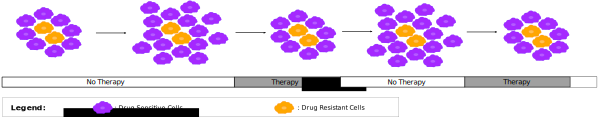
\includegraphics[width=\textwidth]{at}
  \caption{Illustration of control under AT}
  \label{at}
\end{figure}

\section{Importance of competition in adaptive therapy}
The only way of controlling the resistant phenotype for a fixed drug in AT is through competition by the sensitive cells. Therefore, the success of AT in containing the tumour depends on the effectiveness of competition between sensitive and resistant cells. Although, previously it was thought that resistant cells are required to have an inherent disadvantage for AT to be successful, even without it the survival time can be prolonged by competition between the cells \cite{Strobl}.

Cells can use different strategies such as higher proliferation rate, better survival at sub-optimal conditions or lower death rate to compete with each other, and several such strategies are seen to be acquired over the course of cancer progression, as shown by the ``hallmarks of cancer" framework \cite{Hanahan}.

\section{System of Study}
The metastatic castration resistant prostate cancer (mCRPC) was chosen to be the system of study. The mCRPC system already has a history of AT work done on it, although in different contexts \cite{Cunningham,Zhang}.

Prostate cells express androgen receptors (ARs) that require testosterone or its metabolite, 5$\alpha$-dihydrotestosterone to activate. Activated AR bind to promoters of genes responsible for proliferation \cite{Heinlein}. Without testosterone, proliferation is halted and the cells die of apoptosis. When cancerous cells evolve from prostate cells, the AR mechanism is preserved and such prostate cancer remains testosterone dependent.

This system is usually modelled as consisting of three different types of cells: $T^+$, $T^p$ and $T^-$. $T^+$ is the baseline population for prostate cancer which require testosterone for survival. The standard therapy for prostate cancer is castration or androgen deprivation therapy (ADT) which blocks external production of testosterone and would kill the $T^+$ cells in a normal castration sensitive prostate cancer. However, castration resistant prostate cancer soon develops, as the $T^p$ cells can produce testosterone and sustain the $T^+$ cells. $T^p$ cells are also dependent on testosterone, and they produce testosterone from cholesterol through upregulation of CYP17$\alpha$ \cite{Dillard}. The $T^-$ cells on the other hand do not require testosterone as they have mutated ARs that remain active even in the absence of testosterone.

Abiraterone is a drug developed against mCRPC that inhibits the CYP17$\alpha$ and can be effective against both $T^+$ and $T^p$, however, not against $T^-$. And, this could lead to competitive release of the resistant $T^-$ cells if adminitered in the standard clinical protocol. Abiraterone is usually adminitered after ADT as the system develops into a mCRPC. For our study, we shall only consider AT protocols on abiraterone under ADT.

\section{Goal of the Project}
The goal of the project is to:
\begin{enumerate}
  \item Develop a model of the chosen system of study with their respective resource dependence.
  \item Study the dynamics of the system under different conditions in the absence of therapy.
  \item Compare the dynamics under effect of different therapy regimens.
  \item Find the corresponding optimal therapy regimen that maximises the survival time for particular conditions.
\end{enumerate}
